\documentclass{standalone}
\usepackage{tikz}
\usetikzlibrary{patterns, positioning}
\usepackage[sfdefault]{ClearSans} %% option 'sfdefault' activates Clear Sans as the default text font
\usepackage[T1]{fontenc}

\begin{document}
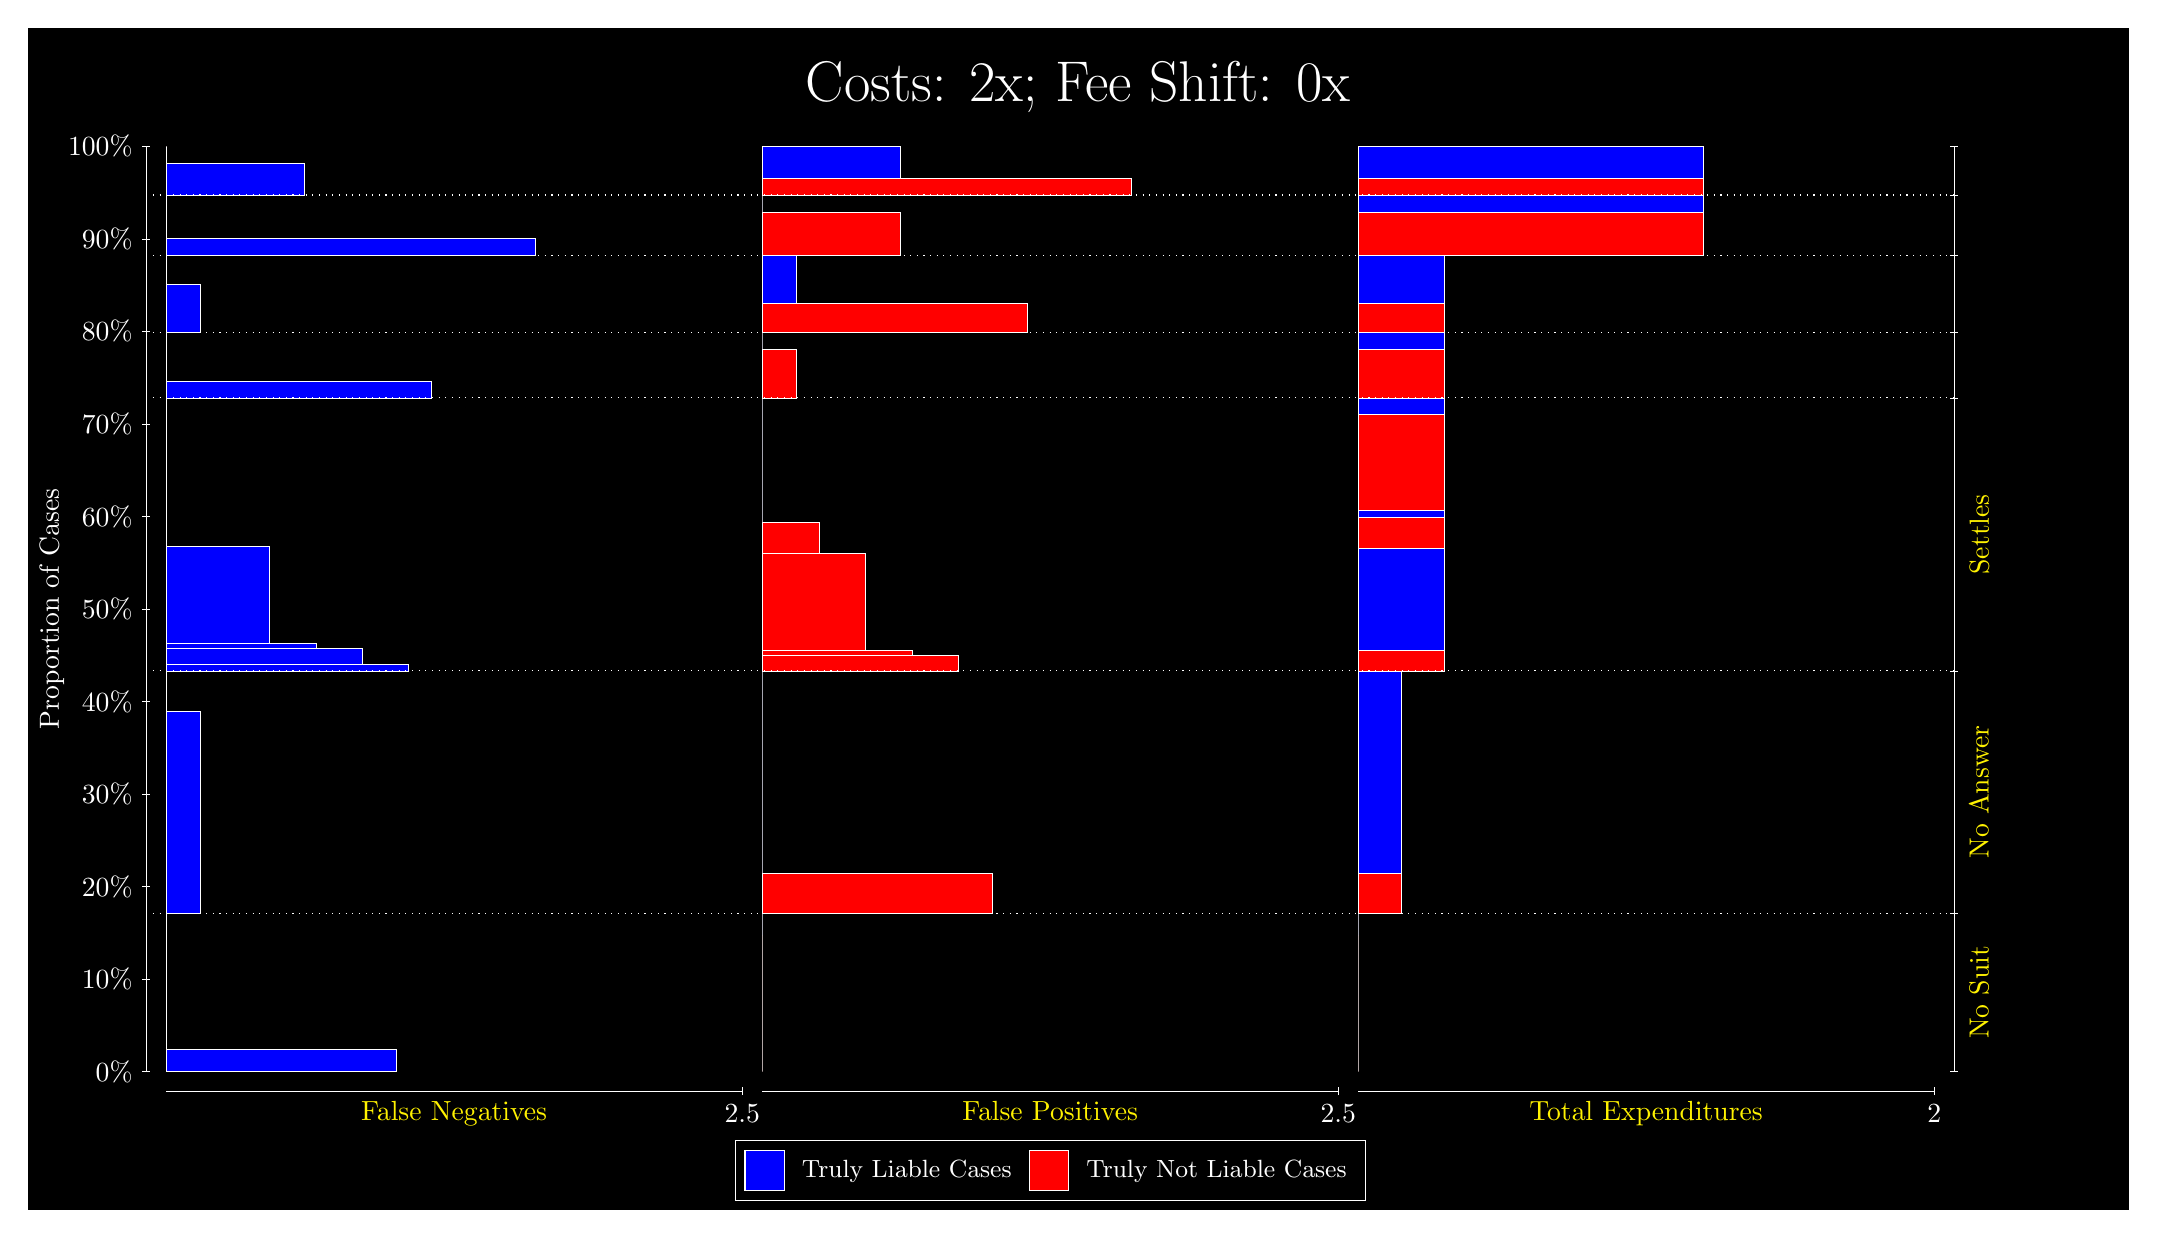
\begin{tikzpicture}
\draw[fill=black] (0,0) rectangle (26.667,15);
\draw[text=white] (0,13.5) rectangle (26.667,15) node[midway] {\huge Costs: 2x; Fee Shift: 0x};
\draw[white, very thin] (1.5,1.75) -- (1.5,13.5);
\node[rotate=90, text=white, anchor=center] at (0.3, 7.625) {Proportion of Cases};
\draw[white, very thin] (1.45,1.75) -- (1.55,1.75);
\node[text=white, anchor=east] at (1.45, 1.75) {0\%};
\draw[white, very thin] (1.45,2.925) -- (1.55,2.925);
\node[text=white, anchor=east] at (1.45, 2.925) {10\%};
\draw[white, very thin] (1.45,4.1) -- (1.55,4.1);
\node[text=white, anchor=east] at (1.45, 4.1) {20\%};
\draw[white, very thin] (1.45,5.275) -- (1.55,5.275);
\node[text=white, anchor=east] at (1.45, 5.275) {30\%};
\draw[white, very thin] (1.45,6.45) -- (1.55,6.45);
\node[text=white, anchor=east] at (1.45, 6.45) {40\%};
\draw[white, very thin] (1.45,7.625) -- (1.55,7.625);
\node[text=white, anchor=east] at (1.45, 7.625) {50\%};
\draw[white, very thin] (1.45,8.8) -- (1.55,8.8);
\node[text=white, anchor=east] at (1.45, 8.8) {60\%};
\draw[white, very thin] (1.45,9.975) -- (1.55,9.975);
\node[text=white, anchor=east] at (1.45, 9.975) {70\%};
\draw[white, very thin] (1.45,11.15) -- (1.55,11.15);
\node[text=white, anchor=east] at (1.45, 11.15) {80\%};
\draw[white, very thin] (1.45,12.325) -- (1.55,12.325);
\node[text=white, anchor=east] at (1.45, 12.325) {90\%};
\draw[white, very thin] (1.45,13.5) -- (1.55,13.5);
\node[text=white, anchor=east] at (1.45, 13.5) {100\%};

\draw[white, very thin] (24.457,1.75) -- (24.457,13.5);
\draw[white, very thin] (24.407,1.75) -- (24.507,1.75);
\node[anchor=west] at (24.407, 1.75) {};
\draw[white, very thin] (24.407,3.7621) -- (24.507,3.7621);
\node[anchor=west] at (24.407, 3.7621) {};
\draw[white, very thin] (24.407,6.838) -- (24.507,6.838);
\node[anchor=west] at (24.407, 6.838) {};
\draw[white, very thin] (24.407,10.306) -- (24.507,10.306);
\node[anchor=west] at (24.407, 10.306) {};
\draw[white, very thin] (24.407,11.136) -- (24.507,11.136);
\node[anchor=west] at (24.407, 11.136) {};
\draw[white, very thin] (24.407,12.115) -- (24.507,12.115);
\node[anchor=west] at (24.407, 12.115) {};
\draw[white, very thin] (24.407,12.882) -- (24.507,12.882);
\node[anchor=west] at (24.407, 12.882) {};
\draw[white, very thin] (24.407,13.5) -- (24.507,13.5);
\node[anchor=west] at (24.407, 13.5) {};

\draw[white, very thin, fill=blue] (1.75,1.75) rectangle (4.6775,2.0313);
\draw[white, very thin, fill=red] (1.75,2.0313) rectangle (1.75,3.7621);
\draw[white, very thin, fill=blue] (1.75,3.7621) rectangle (2.1891,6.3306);
\draw[white, very thin, fill=red] (1.75,6.3306) rectangle (1.75,6.838);
\draw[white, very thin, fill=blue] (1.75,6.838) rectangle (4.8239,6.9249);
\draw[white, very thin, fill=blue] (1.75,6.9249) rectangle (4.2384,7.1282);
\draw[white, very thin, fill=blue] (1.75,7.1282) rectangle (3.6529,7.1922);
\draw[white, very thin, fill=blue] (1.75,7.1922) rectangle (3.0674,8.4188);
\draw[white, very thin, fill=red] (1.75,8.4188) rectangle (1.75,10.306);
\draw[white, very thin, fill=blue] (1.75,10.306) rectangle (5.1167,10.519);
\draw[white, very thin, fill=red] (1.75,10.519) rectangle (1.75,11.136);
\draw[white, very thin, fill=blue] (1.75,11.136) rectangle (2.1891,11.75);
\draw[white, very thin, fill=red] (1.75,11.75) rectangle (1.75,12.115);
\draw[white, very thin, fill=blue] (1.75,12.115) rectangle (6.4341,12.332);
\draw[white, very thin, fill=red] (1.75,12.332) rectangle (1.75,12.882);
\draw[white, very thin, fill=blue] (1.75,12.882) rectangle (3.5065,13.284);
\draw[white, very thin, fill=red] (1.75,13.284) rectangle (1.75,13.5);
\draw[white, very thin, fill=red] (9.3189,1.75) rectangle (9.3189,3.4808);
\draw[white, very thin, fill=blue] (9.3189,3.4808) rectangle (9.3189,3.7621);
\draw[white, very thin, fill=red] (9.3189,3.7621) rectangle (12.246,4.2695);
\draw[white, very thin, fill=blue] (9.3189,4.2695) rectangle (9.3189,6.838);
\draw[white, very thin, fill=red] (9.3189,6.838) rectangle (11.807,7.0413);
\draw[white, very thin, fill=red] (9.3189,7.0413) rectangle (11.222,7.1054);
\draw[white, very thin, fill=red] (9.3189,7.1054) rectangle (10.636,8.332);
\draw[white, very thin, fill=red] (9.3189,8.332) rectangle (10.051,8.7253);
\draw[white, very thin, fill=blue] (9.3189,8.7253) rectangle (9.3189,10.306);
\draw[white, very thin, fill=red] (9.3189,10.306) rectangle (9.758,10.924);
\draw[white, very thin, fill=blue] (9.3189,10.924) rectangle (9.3189,11.136);
\draw[white, very thin, fill=red] (9.3189,11.136) rectangle (12.686,11.502);
\draw[white, very thin, fill=blue] (9.3189,11.502) rectangle (9.758,12.115);
\draw[white, very thin, fill=red] (9.3189,12.115) rectangle (11.075,12.666);
\draw[white, very thin, fill=blue] (9.3189,12.666) rectangle (9.3189,12.882);
\draw[white, very thin, fill=red] (9.3189,12.882) rectangle (14.003,13.098);
\draw[white, very thin, fill=blue] (9.3189,13.098) rectangle (11.075,13.5);
\draw[white, very thin, fill=red] (16.888,1.75) rectangle (16.888,3.4808);
\draw[white, very thin, fill=blue] (16.888,3.4808) rectangle (16.888,3.7621);
\draw[white, very thin, fill=red] (16.888,3.7621) rectangle (17.437,4.2695);
\draw[white, very thin, fill=blue] (16.888,4.2695) rectangle (17.437,6.838);
\draw[white, very thin, fill=red] (16.888,6.838) rectangle (17.986,7.1054);
\draw[white, very thin, fill=blue] (16.888,7.1054) rectangle (17.986,8.396);
\draw[white, very thin, fill=red] (16.888,8.396) rectangle (17.986,8.7893);
\draw[white, very thin, fill=blue] (16.888,8.7893) rectangle (17.986,8.8762);
\draw[white, very thin, fill=red] (16.888,8.8762) rectangle (17.986,10.103);
\draw[white, very thin, fill=blue] (16.888,10.103) rectangle (17.986,10.306);
\draw[white, very thin, fill=red] (16.888,10.306) rectangle (17.986,10.924);
\draw[white, very thin, fill=blue] (16.888,10.924) rectangle (17.986,11.136);
\draw[white, very thin, fill=red] (16.888,11.136) rectangle (17.986,11.502);
\draw[white, very thin, fill=blue] (16.888,11.502) rectangle (17.986,12.115);
\draw[white, very thin, fill=red] (16.888,12.115) rectangle (21.279,12.666);
\draw[white, very thin, fill=blue] (16.888,12.666) rectangle (21.279,12.882);
\draw[white, very thin, fill=red] (16.888,12.882) rectangle (21.279,13.098);
\draw[white, very thin, fill=blue] (16.888,13.098) rectangle (21.279,13.5);
\draw[white, dotted] (1.5,3.7621) -- (24.457,3.7621);
\draw[white, dotted] (1.5,6.838) -- (24.457,6.838);
\draw[white, dotted] (1.5,10.306) -- (24.457,10.306);
\draw[white, dotted] (1.5,11.136) -- (24.457,11.136);
\draw[white, dotted] (1.5,12.115) -- (24.457,12.115);
\draw[white, dotted] (1.5,12.882) -- (24.457,12.882);
\draw[white, very thin] (1.75,1.5) -- (9.0689,1.5);
\node[text=yellow, anchor=north] at (5.4094, 1.5) {False Negatives};
\draw[white, very thin] (9.0689,1.45) -- (9.0689,1.55);
\node[text=white, anchor=north] at (9.0689, 1.45) {2.5};

\draw[white, very thin] (9.3189,1.5) -- (16.638,1.5);
\node[text=yellow, anchor=north] at (12.978, 1.5) {False Positives};
\draw[white, very thin] (16.638,1.45) -- (16.638,1.55);
\node[text=white, anchor=north] at (16.638, 1.45) {2.5};

\draw[white, very thin] (16.888,1.5) -- (24.207,1.5);
\node[text=yellow, anchor=north] at (20.547, 1.5) {Total Expenditures};
\draw[white, very thin] (24.207,1.45) -- (24.207,1.55);
\node[text=white, anchor=north] at (24.207, 1.45) {2};

\node[text=yellow, centered, rotate=90] at (24.777, 2.7561) {No Suit};
\node[text=yellow, centered, rotate=90] at (24.777, 5.3001) {No Answer};
\node[text=yellow, centered, rotate=90] at (24.777, 8.5721) {Settles};





\draw (12.978300999999998,1.5) node[draw=none] (baseCoordinate) {};
\begin{scope}[align=center]
        \matrix[scale=0.5, draw=white, below=0.5cm of baseCoordinate, nodes={draw}, column sep=0.1cm]{
            \node[rectangle, draw, minimum width=0.5cm, minimum height=0.5cm, fill=blue] {}; &
            \node[draw=none, font=\small, text=white] (B) {Truly Liable Cases}; &
            \node[rectangle, draw, minimum width=0.5cm, minimum height=0.5cm, fill=red] {}; &
            \node[draw=none, font=\small, text=white] (B) {Truly Not Liable Cases}; \\
            };
\end{scope}

\end{tikzpicture}
\end{document}